% -*- mode: noweb; noweb-default-code-mode: R-mode; -*-
\documentclass[a4paper]{article}

\usepackage{a4wide}
\usepackage{lscape}
\usepackage[margin=.2in]{geometry}

\title{Heritability by Subgroup}
\author{Joe Rodger's BG Team}

\usepackage{Sweave}
\begin{document}
\maketitle
Gen2 Link Version: 2011V28.

%%%%%%%%
% Here is some text that is rendered almost explictly
%%%%%%%%

Subjects were 19+ years old.  Implicit ambiguous sibs were assigned R=0.375. Z-Scores are restricted to  +/-10.

Counts reflect the double entry.
% latex table generated in R 2.14.0 by xtable 1.6-0 package
% Wed Dec 14 20:04:25 2011
\begin{table}[ht]
\begin{center}
\begin{tabular}{lr|rrr|rrr|rrrrr|rrrr}
 Subgroup & $N$ & $h^2$ & $c^2$ & $e^2$ & $\bar{X}$ & $\sigma$ & $\sigma^3$ & $N_{.25}$ & $N_{.375}$ & $N_{.5}$ & $N_{.75}$ & $N_{Mz}$ & $r_{.25}$ & $r_{.375}$ & $r_{.5}$ & $r_{Mz}$ \\ 
 Total & 7098 & 0.72 & 0.04 & 0.24 & -0.03 & 1.01 & -0.03 & 2206 & 0 & 4864 & 0 & 28 & 0.23 &  & 0.40 & 0.94 \\ 
   \hline
FF & 1770 & 0.84 & 0.04 & 0.12 & -0.05 & 1.02 & 0.04 & 574 & 0 & 1186 & 0 & 10 & 0.25 &  & 0.46 & 0.95 \\ 
  MF & 3532 & 0.66 & 0.05 & 0.29 & 0.00 & 1.02 & -0.06 & 1110 & 0 & 2422 & 0 & 0 & 0.22 &  & 0.38 &  \\ 
  MM & 1796 & 0.73 & 0.01 & 0.27 & -0.07 & 0.99 & -0.03 & 522 & 0 & 1256 & 0 & 18 & 0.20 &  & 0.36 & 0.94 \\ 
   \hline
Hispanic & 1778 & 0.23 & 0.29 & 0.48 & -0.40 & 0.96 & 0.13 & 404 & 0 & 1372 & 0 & 2 & 0.36 &  & 0.40 & -1.00 \\ 
  Black & 2898 & 0.68 & -0.03 & 0.35 & -0.02 & 1.01 & 0.00 & 1380 & 0 & 1508 & 0 & 10 & 0.15 &  & 0.31 & 0.88 \\ 
  NBNH & 2422 & 0.50 & 0.11 & 0.39 & 0.24 & 0.96 & -0.17 & 422 & 0 & 1984 & 0 & 16 & 0.25 &  & 0.35 & 0.95 \\ 
   \hline
Hisp FF & 410 & -0.07 & 0.48 & 0.58 & -0.45 & 0.93 & 0.23 & 108 & 0 & 302 & 0 & 0 & 0.47 &  & 0.45 &  \\ 
  Hisp MF & 852 & 0.32 & 0.23 & 0.45 & -0.36 & 0.99 & 0.14 & 196 & 0 & 656 & 0 & 0 & 0.31 &  & 0.39 &  \\ 
  Hisp MM & 516 & 0.39 & 0.21 & 0.40 & -0.44 & 0.93 & 0.01 & 100 & 0 & 414 & 0 & 2 & 0.34 &  & 0.39 & -1.00 \\ 
   \hline
Black FF & 778 & 0.62 & 0.02 & 0.36 & -0.02 & 1.03 & -0.04 & 382 & 0 & 392 & 0 & 4 & 0.18 &  & 0.32 & 0.80 \\ 
  Black MF & 1450 & 0.72 & -0.03 & 0.30 & -0.00 & 1.02 & -0.01 & 690 & 0 & 760 & 0 & 0 & 0.15 &  & 0.34 &  \\ 
  Black MM & 670 & 0.69 & -0.11 & 0.42 & -0.05 & 0.97 & 0.07 & 308 & 0 & 356 & 0 & 6 & 0.08 &  & 0.20 & 0.89 \\ 
   \hline
NBNH FF & 582 & 1.00 & -0.02 & 0.02 & 0.19 & 0.98 & 0.00 & 84 & 0 & 492 & 0 & 6 & 0.23 &  & 0.48 & 0.97 \\ 
  NBNH MF & 1230 & 0.31 & 0.16 & 0.53 & 0.26 & 0.96 & -0.23 & 224 & 0 & 1006 & 0 & 0 & 0.23 &  & 0.31 &  \\ 
  NBNH MM & 610 & 0.29 & 0.17 & 0.55 & 0.22 & 0.96 & -0.23 & 114 & 0 & 486 & 0 & 10 & 0.28 &  & 0.29 & 0.94 \\ 
  \end{tabular}
\caption{Height Heritability}
\label{tab:two}
\end{center}
\end{table}%\end{landscape}
%%%%%%%%%%%%%%%%%%%%%%%%%%%%%%%%%%%%%%%%%%%%%%%%%%%%%%%%%%%%%%%%%%%%%%
% Get the results for the graphs
%%%%%%%%%%%%%%%%%%%%%%%%%%%%%%%%%%%%%%%%%%%%%%%%%%%%%%%%%%%%%%%%%%%%%%
%Total
 %Default size for remaining graphs
\section{Total Sample}
\begin{figure}[htbp]
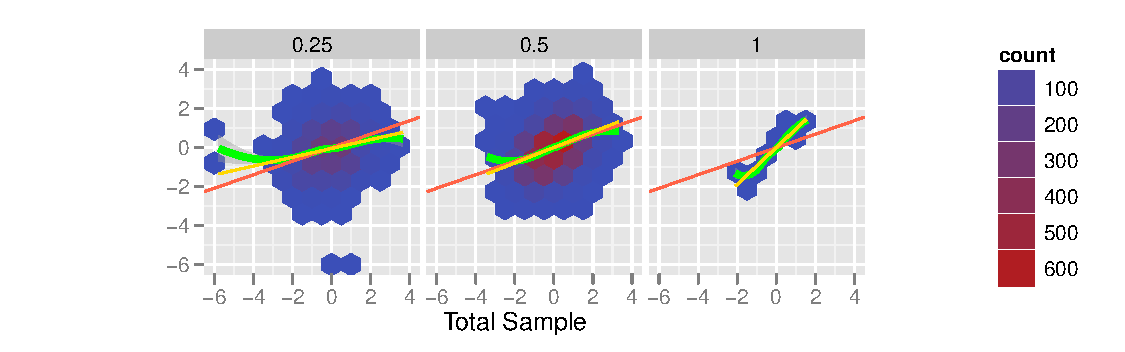
\includegraphics{Height-004}
\end{figure}
Plot Explanation: Each row of graphs isolates a subgroup.  

Each cell in a row isolates a unique value of R; this is displayed in the gray header above each cell. 

Axis and hexbin sizes are constants across all rows.

The orange line is the LS regression for the row (repeated in each cell).

The yellow line is the LS regression for the cell.

The green line is the loess for each cell.  It's bandwidth is not constant across allrows.

The hexbin density color is not constant across rows.

Relevant portions of the table are repeated on each page.
\newpage
\section{By Gender}
% latex table generated in R 2.14.0 by xtable 1.6-0 package
% Wed Dec 14 20:04:29 2011
\begin{table}[ht]
\begin{center}
\begin{tabular}{l|rrr|rrrrr|rrrr}
 Subgroup & $h^2$ & $c^2$ & $e^2$ & $N_{.25}$ & $N_{.375}$ & $N_{.5}$ & $N_{.75}$ & $N_{Mz}$ & $r_{.25}$ & $r_{.375}$ & $r_{.5}$ & $r_{Mz}$ \\ 
 Total & 0.72 & 0.04 & 0.24 & 2206 &   0 & 4864 &   0 &  28 & 0.23 &  & 0.40 & 0.94 \\ 
   \hline
FF & 0.84 & 0.04 & 0.12 & 574 &   0 & 1186 &   0 &  10 & 0.25 &  & 0.46 & 0.95 \\ 
  MF & 0.66 & 0.05 & 0.29 & 1110 &   0 & 2422 &   0 &   0 & 0.22 &  & 0.38 &  \\ 
  MM & 0.73 & 0.01 & 0.27 & 522 &   0 & 1256 &   0 &  18 & 0.20 &  & 0.36 & 0.94 \\ 
  \end{tabular}
\end{center}
\end{table}\begin{figure}[htbp]
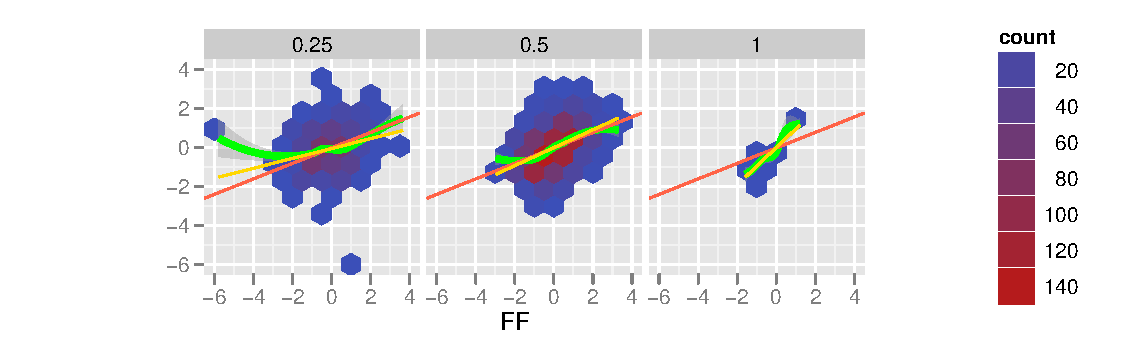
\includegraphics{Height-006}
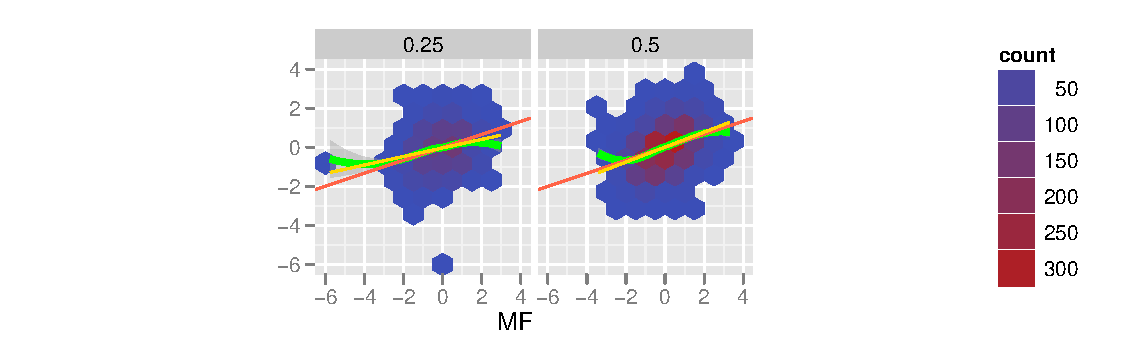
\includegraphics{Height-007}
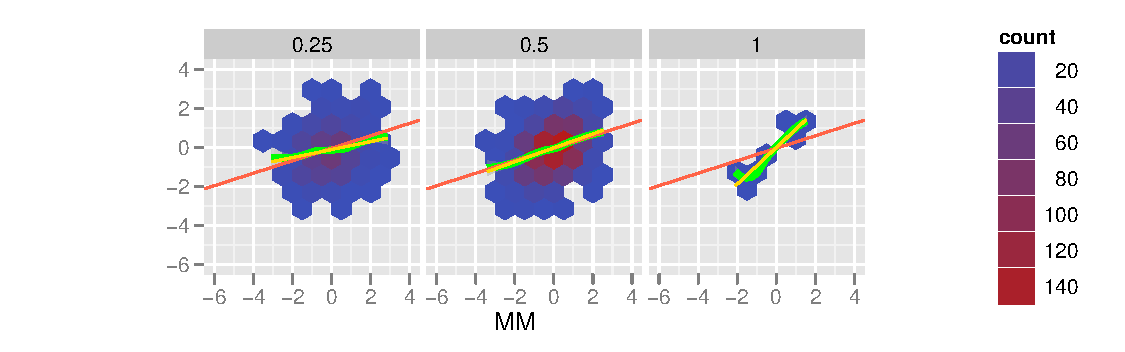
\includegraphics{Height-008}
\end{figure}

\newpage
\section{By Race}
% latex table generated in R 2.14.0 by xtable 1.6-0 package
% Wed Dec 14 20:04:35 2011
\begin{table}[ht]
\begin{center}
\begin{tabular}{l|rrr|rrrrr|rrrr}
 Subgroup & $h^2$ & $c^2$ & $e^2$ & $N_{.25}$ & $N_{.375}$ & $N_{.5}$ & $N_{.75}$ & $N_{Mz}$ & $r_{.25}$ & $r_{.375}$ & $r_{.5}$ & $r_{Mz}$ \\ 
 Total & 0.72 & 0.04 & 0.24 & 2206 &   0 & 4864 &   0 &  28 & 0.23 &  & 0.40 & 0.94 \\ 
   \hline
Hispanic & 0.23 & 0.29 & 0.48 & 404 &   0 & 1372 &   0 &   2 & 0.36 &  & 0.40 & -1.00 \\ 
  Black & 0.68 & -0.03 & 0.35 & 1380 &   0 & 1508 &   0 &  10 & 0.15 &  & 0.31 & 0.88 \\ 
  NBNH & 0.50 & 0.11 & 0.39 & 422 &   0 & 1984 &   0 &  16 & 0.25 &  & 0.35 & 0.95 \\ 
  \end{tabular}
\end{center}
\end{table}\begin{figure}[htbp]
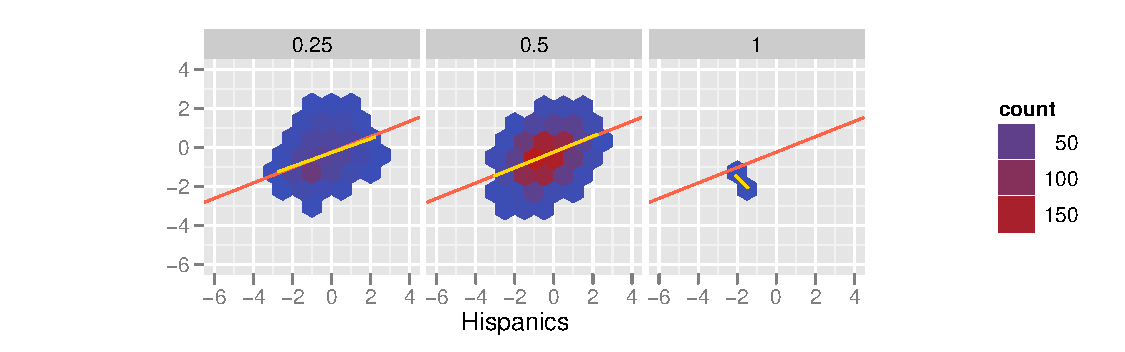
\includegraphics{Height-010}
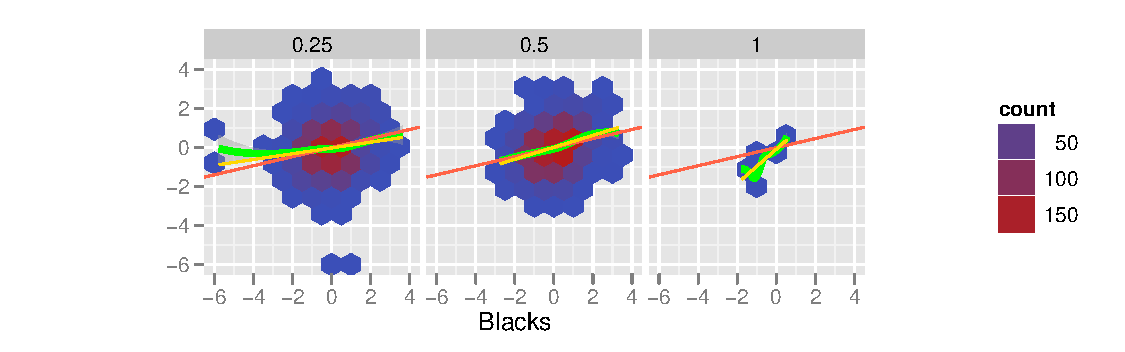
\includegraphics{Height-011}
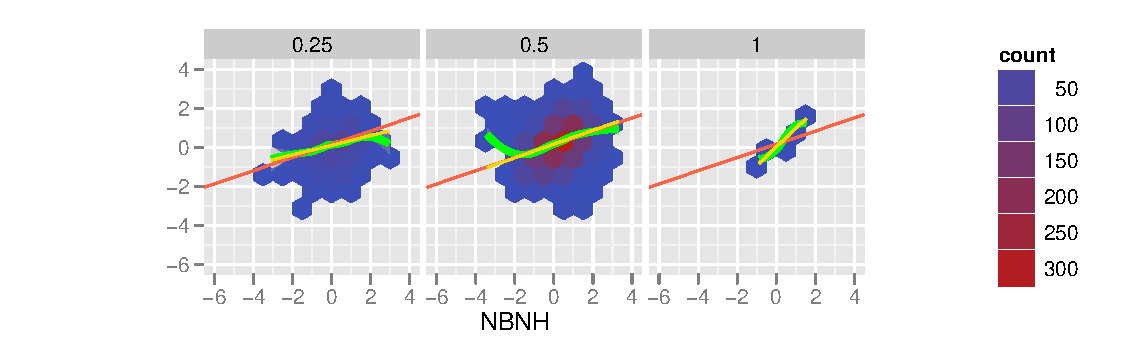
\includegraphics{Height-012}
\end{figure}

\newpage
\section{By Gender for Hispanics}
% latex table generated in R 2.14.0 by xtable 1.6-0 package
% Wed Dec 14 20:04:40 2011
\begin{table}[ht]
\begin{center}
\begin{tabular}{l|rrr|rrrrr|rrrr}
 Subgroup & $h^2$ & $c^2$ & $e^2$ & $N_{.25}$ & $N_{.375}$ & $N_{.5}$ & $N_{.75}$ & $N_{Mz}$ & $r_{.25}$ & $r_{.375}$ & $r_{.5}$ & $r_{Mz}$ \\ 
 Total & 0.72 & 0.04 & 0.24 & 2206 &   0 & 4864 &   0 &  28 & 0.23 &  & 0.40 & 0.94 \\ 
   \hline
Hispanic & 0.23 & 0.29 & 0.48 & 404 &   0 & 1372 &   0 &   2 & 0.36 &  & 0.40 & -1.00 \\ 
  Hisp FF & -0.07 & 0.48 & 0.58 & 108 &   0 & 302 &   0 &   0 & 0.47 &  & 0.45 &  \\ 
  Hisp MF & 0.32 & 0.23 & 0.45 & 196 &   0 & 656 &   0 &   0 & 0.31 &  & 0.39 &  \\ 
  Hisp MM & 0.39 & 0.21 & 0.40 & 100 &   0 & 414 &   0 &   2 & 0.34 &  & 0.39 & -1.00 \\ 
  \end{tabular}
\end{center}
\end{table}\begin{figure}[htbp]
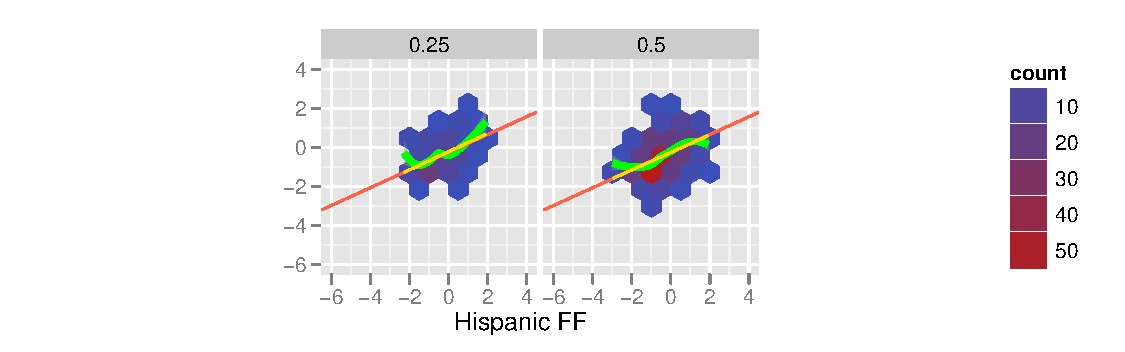
\includegraphics{Height-014}
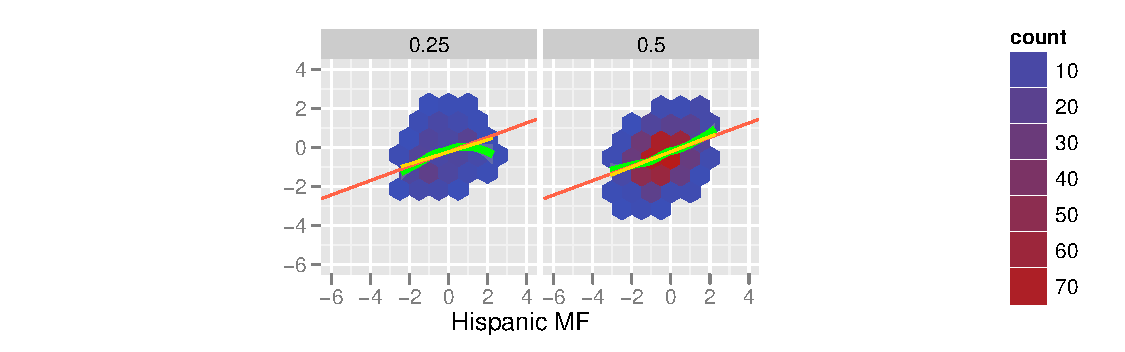
\includegraphics{Height-015}
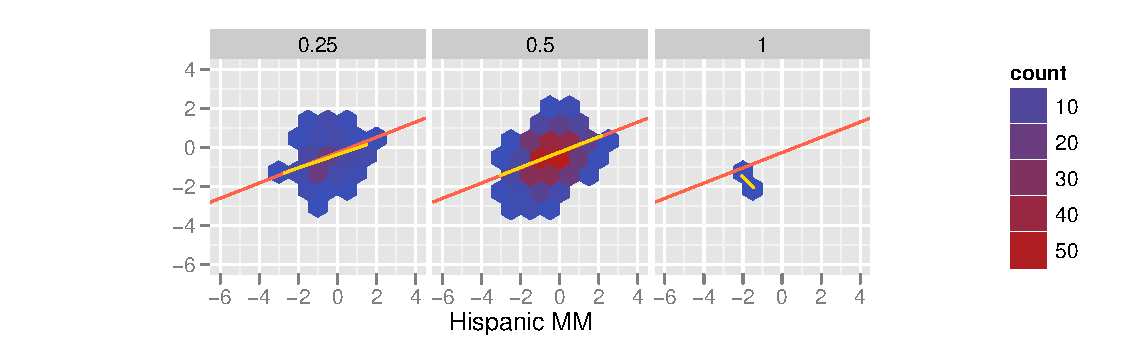
\includegraphics{Height-016}
\end{figure}

\newpage
\section{By Gender for Blacks}
% latex table generated in R 2.14.0 by xtable 1.6-0 package
% Wed Dec 14 20:04:44 2011
\begin{table}[ht]
\begin{center}
\begin{tabular}{l|rrr|rrrrr|rrrr}
 Subgroup & $h^2$ & $c^2$ & $e^2$ & $N_{.25}$ & $N_{.375}$ & $N_{.5}$ & $N_{.75}$ & $N_{Mz}$ & $r_{.25}$ & $r_{.375}$ & $r_{.5}$ & $r_{Mz}$ \\ 
 Total & 0.72 & 0.04 & 0.24 & 2206 &   0 & 4864 &   0 &  28 & 0.23 &  & 0.40 & 0.94 \\ 
   \hline
Black & 0.68 & -0.03 & 0.35 & 1380 &   0 & 1508 &   0 &  10 & 0.15 &  & 0.31 & 0.88 \\ 
  Black FF & 0.62 & 0.02 & 0.36 & 382 &   0 & 392 &   0 &   4 & 0.18 &  & 0.32 & 0.80 \\ 
  Black MF & 0.72 & -0.03 & 0.30 & 690 &   0 & 760 &   0 &   0 & 0.15 &  & 0.34 &  \\ 
  Black MM & 0.69 & -0.11 & 0.42 & 308 &   0 & 356 &   0 &   6 & 0.08 &  & 0.20 & 0.89 \\ 
  \end{tabular}
\end{center}
\end{table}\begin{figure}[htbp]
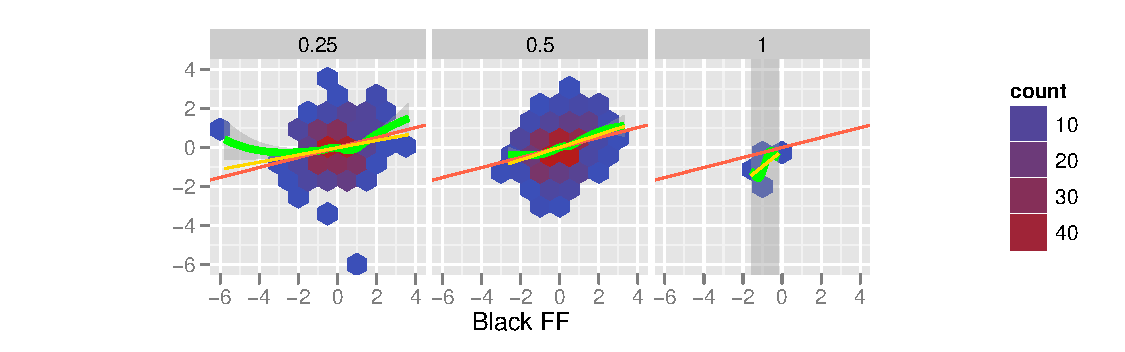
\includegraphics{Height-018}
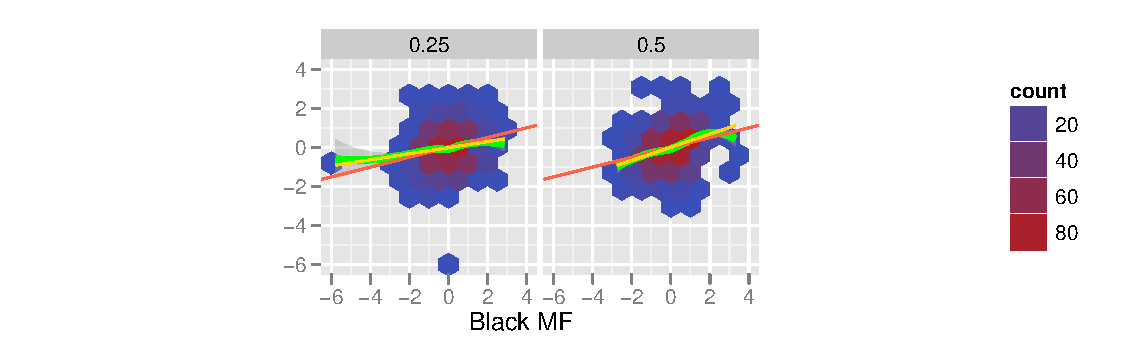
\includegraphics{Height-019}
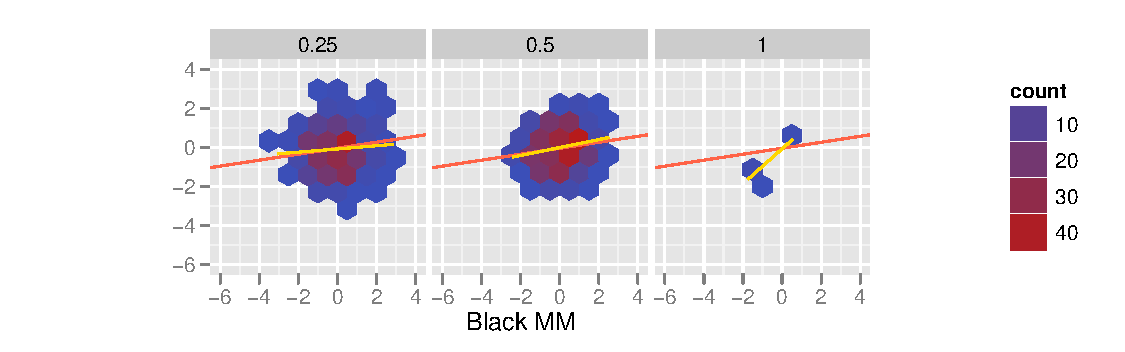
\includegraphics{Height-020}
\end{figure}

\newpage
\section{By Gender for NBNHs}
% latex table generated in R 2.14.0 by xtable 1.6-0 package
% Wed Dec 14 20:04:48 2011
\begin{table}[ht]
\begin{center}
\begin{tabular}{l|rrr|rrrrr|rrrr}
 Subgroup & $h^2$ & $c^2$ & $e^2$ & $N_{.25}$ & $N_{.375}$ & $N_{.5}$ & $N_{.75}$ & $N_{Mz}$ & $r_{.25}$ & $r_{.375}$ & $r_{.5}$ & $r_{Mz}$ \\ 
 Total & 0.72 & 0.04 & 0.24 & 2206 &   0 & 4864 &   0 &  28 & 0.23 &  & 0.40 & 0.94 \\ 
   \hline
NBNH & 0.50 & 0.11 & 0.39 & 422 &   0 & 1984 &   0 &  16 & 0.25 &  & 0.35 & 0.95 \\ 
  NBNH FF & 1.00 & -0.02 & 0.02 &  84 &   0 & 492 &   0 &   6 & 0.23 &  & 0.48 & 0.97 \\ 
  NBNH MF & 0.31 & 0.16 & 0.53 & 224 &   0 & 1006 &   0 &   0 & 0.23 &  & 0.31 &  \\ 
  NBNH MM & 0.29 & 0.17 & 0.55 & 114 &   0 & 486 &   0 &  10 & 0.28 &  & 0.29 & 0.94 \\ 
  \end{tabular}
\end{center}
\end{table}\begin{figure}[htbp]
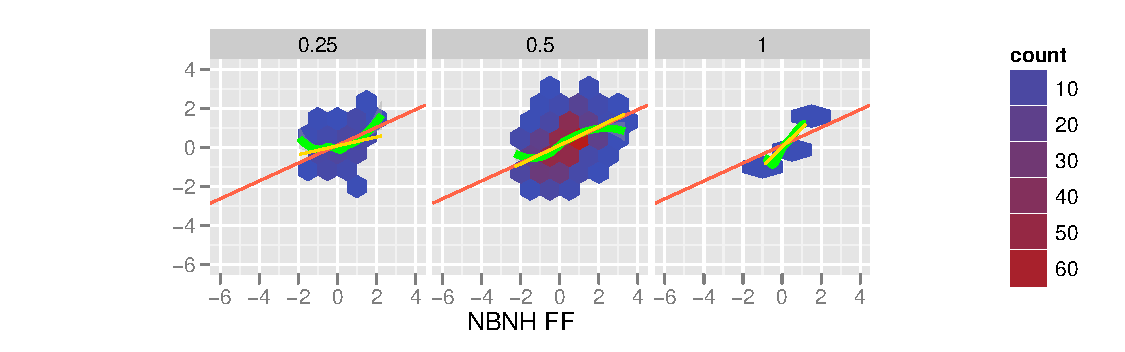
\includegraphics{Height-022}
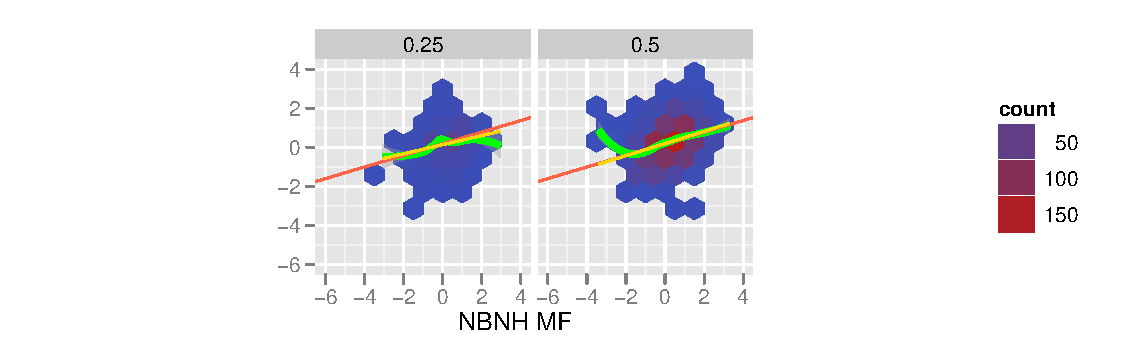
\includegraphics{Height-023}
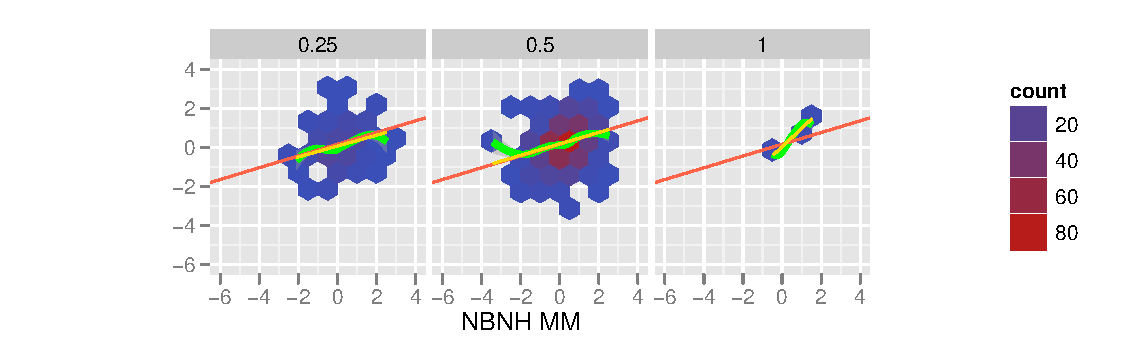
\includegraphics{Height-024}
\end{figure}


\end{document}
